\section{Optimised Implementation}
In order to optimise the na\"ive implementation the execution time for each line was investigated using line_profiler. The result of running the line_profiler on the na\"ive implementation can be seen in \autoref{AppLinePS1}. As can be seen in \autoref{AppLinePS1} the line that takes the absolute longest to execute per hit are the lines which calls the function that creates the histograms. Therefore, this was the first thing to be improved. This was done by utilising the Numpy function for generating histograms. Once this was done the script was much faster as can be seen in \autoref{AppLinePS2}. However, when inspecting the histograms after this alteration it seemed an issue had been introduced. The histogram showed that certain bins were eliminated, as can be seen in \autoref{fig:HistEli}. 
\begin{figure}[h]
\centering
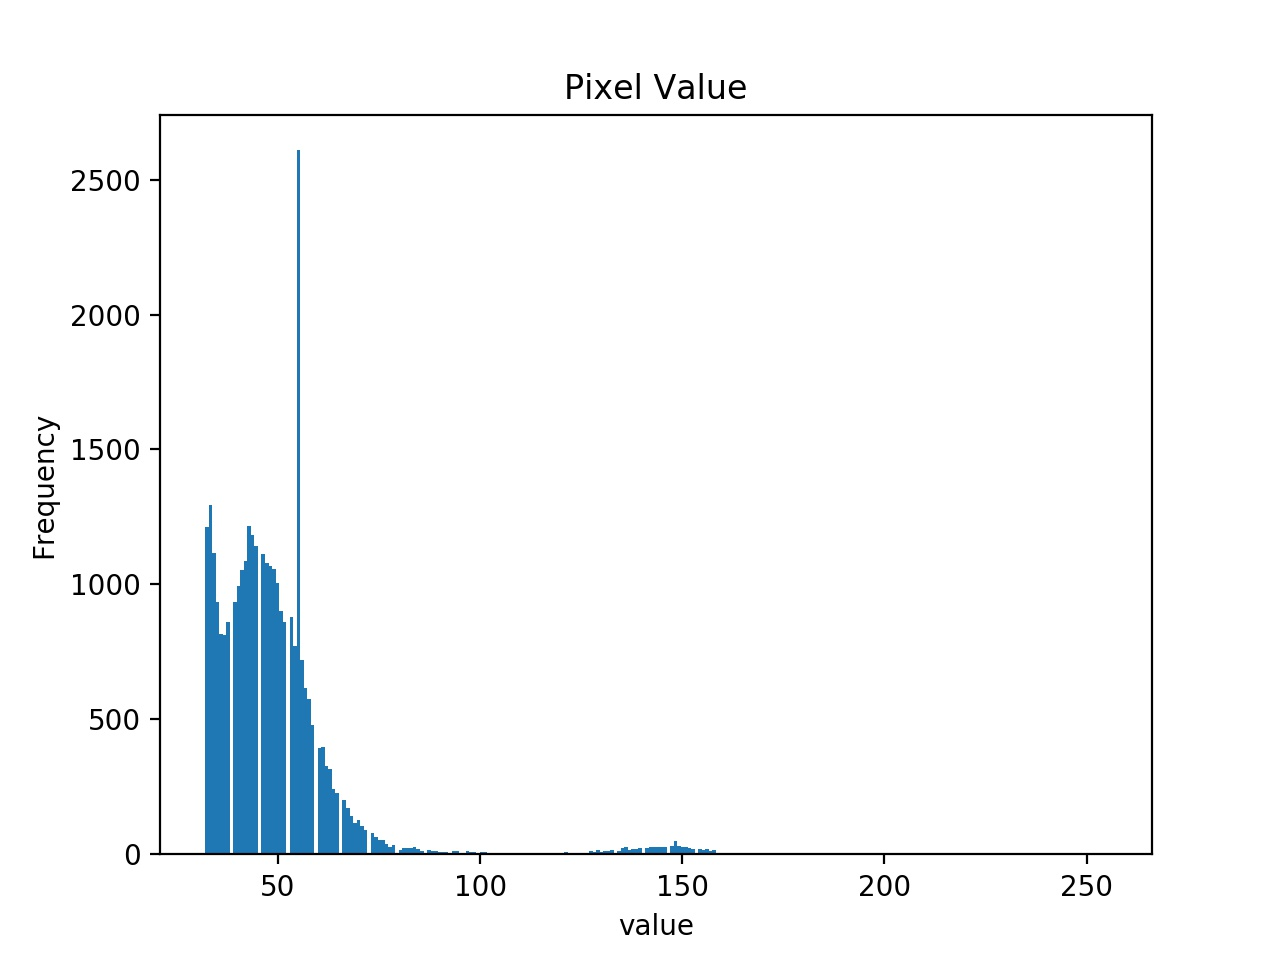
\includegraphics[width=\textwidth]{figures/hist_troublespacing.jpg}
\caption{The histogram of the reconstructed image with eliminated values.}
\label{fig:HistEli}
\end{figure}
\noindent
Eventually it turned out that this was due to the fact that the numpy.histogram adapts the range of the histogram to the range of the present values if no range is specified. This was easily solved by passing an range as an argument to the histogram function. The range in this case had to be specified as range(0,256)

The final source code of the optimised can be found in \autoref{AppOpt}